\documentclass{beamer}

\usepackage[utf8]{inputenc}
\usepackage{beamertheme_atilla/beamerthemeAtilla}
\usepackage{listings}

\institute{E.I.S.T.I.}
\title{L'histoire de 0x5f3759df}
\author{Clément Villain}
\date{\today}

\begin{document}

\begin{frame}[t,plain]
\titlepage
\end{frame}

\section{Préambule}

\begin{frame}{Fast inverse square root}
\begin{figure}
\centering
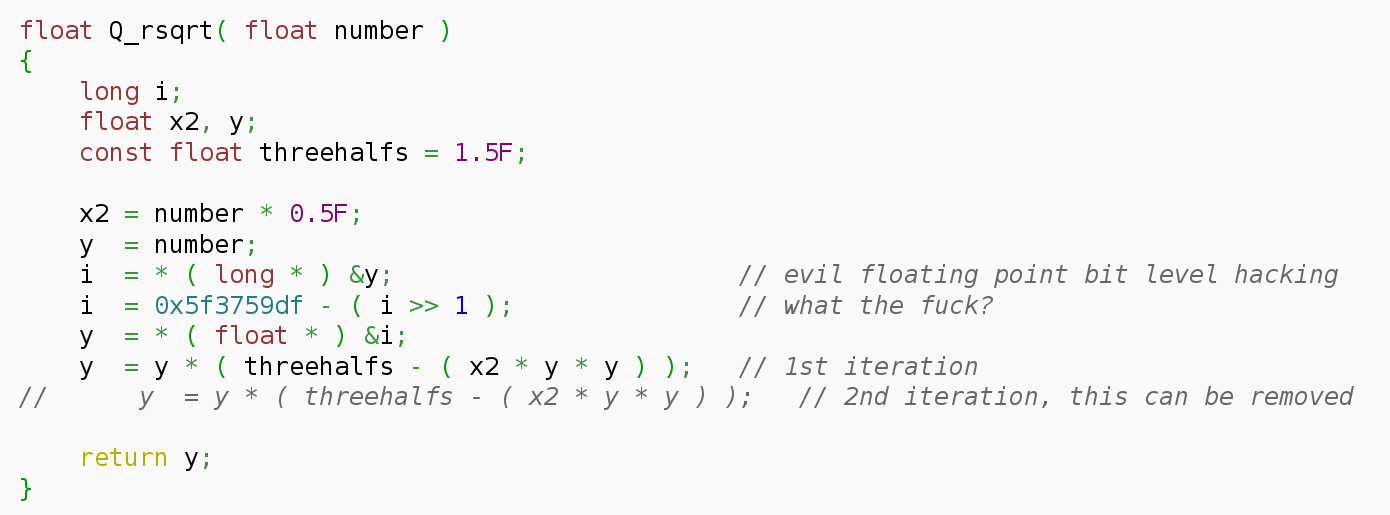
\includegraphics[scale=0.23]{img/code.png}
\caption{Code source de \textit{Quake III Arena}}
\end{figure}
\end{frame}

\begin{frame}{Prérequis: Représentation des nombres}
\begin{figure}
\centering
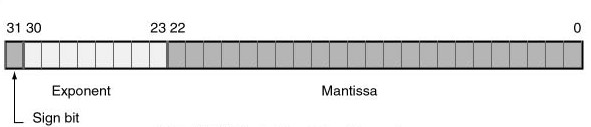
\includegraphics[scale=0.5]{img/i3e.jpg}
\caption{Réprésentation IEEE 754: float}
\end{figure}

\begin{itemize}
\item Valeur d'un float $x = 2^e(1 + m)$ avec $e = E - B$ et $B = 127$
\item Réprésentation entière: $X = M + LE$ avec $m = \frac{M}{L}$ et $L = 2^{23}$
\end{itemize}
\end{frame}

\section{Des mathématiques}
\begin{frame}{Calcul de $\frac{1}{\sqrt{x}}$}
\begin{enumerate}
\item Passage au $\log_2$: 
\begin{center}
 $y = \frac{1}{\sqrt{x}}$ donc  $\log_2(y) = -\frac{1}{2}\log_2(x)$
\end{center}
\item Réprésentation flottante:
$$\log_2(1 + m_y) + e_y = -\frac{1}{2}(\log_2(1 + m_x) + e_x)$$
\item DL du $log_2$:
$$m_y + \sigma + e_y \simeq -\frac{1}{2}(m_x + \sigma + e_x)$$
\item Réprésentation entière: \\
\begin{center}
$m = \frac{M}{L}$ et $e = E - B$
\end{center}
\item Finalement:
$$ I_y \simeq \frac{3}{2}L(B - \sigma) -\frac{1}{2}I_x ~~~~~~~~~~~~~~~~~~~~~~~~~~~$$
\end{enumerate}
\end{frame}

\begin{frame}{Comment choisir $\sigma$}
Pour $\sigma = 0.0450465$
\begin{figure}
\center
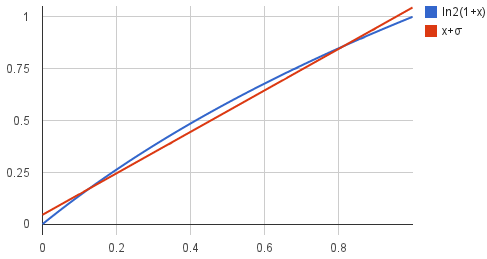
\includegraphics[scale=0.5]{img/ln.png}
\caption{Approximation de $\log_2(1 + x)$}
\end{figure}
\end{frame}

\section{Conclusion}

\begin{frame}{Notre nombre magique}
Rappel:
$$ I_y \simeq \frac{3}{2}L(B - \sigma) -\frac{1}{2}I_x $$

$\frac{3}{2}2^{23}(127  - 0.0450465) = $ 0x5f3759df
\begin{figure}

\includegraphics[scale=0.5]{img/magic.png}
\caption{Application de la formule}
\end{figure}

\end{frame}

\begin{frame}{Performance}
\begin{figure}
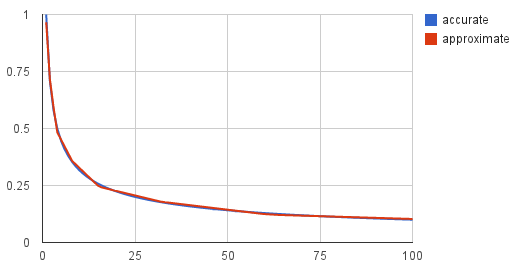
\includegraphics[scale=0.4]{img/res.png}
\caption{Qualité de l'approximation}
\end{figure}
Efficace, rapide et généralisable
\end{frame}
 
\begin{frame}{C'est fini !}
	\begin{huge}
	En espérant vous voir nombreux pour les talks fin janvier !
	\end{huge}
	\begin{figure}
	
\includegraphics[scale=0.1]{img/logo-atilla.png}	
	\end{figure}

\end{frame} 
 
\end{document}
